% Copyright (c) 2026 Jonathan Yantis. SPDX-License-Identifier: CC-BY-4.0
\documentclass[10pt,letterpaper]{article}
\usepackage[margin=.74in,headsep=.19in]{geometry}
\usepackage[T1]{fontenc}
\usepackage{lmodern,microtype,amsmath,amssymb,booktabs,array,ragged2e,xcolor,tikz,listings,enumitem,fancyhdr,xurl}
\usetikzlibrary{arrows.meta,positioning,calc}
\definecolor{ink}{HTML}{24465B}
\definecolor{pale}{HTML}{EEF3F5}
\definecolor{accent}{HTML}{A35C35}
\usepackage[colorlinks=true,allcolors=ink]{hyperref}
\newcommand{\src}[1]{\nolinkurl{#1}}
\newcommand{\ns}{\,\mathrm{ns}}
\newcommand{\us}{\,\mu\mathrm{s}}
\newcommand{\ms}{\,\mathrm{ms}}
\newcommand{\pin}{\texttt{a9ae0294cd8f}}
\newcolumntype{L}[1]{>{\RaggedRight\arraybackslash}p{#1}}
\setlength{\parindent}{0pt}
\setlength{\parskip}{4pt}
\setlength{\headheight}{14pt}
\setlength{\emergencystretch}{2em}
\setlength{\tabcolsep}{5pt}
\setlist{nosep,leftmargin=1.4em}
\widowpenalty=10000\clubpenalty=10000
\lstset{basicstyle=\ttfamily\small,columns=fullflexible,keepspaces=true,showstringspaces=false,
 frame=single,rulecolor=\color{ink!30},backgroundcolor=\color{pale},xleftmargin=4pt,xrightmargin=4pt,
 aboveskip=6pt,belowskip=6pt,breaklines=true}
\pagestyle{fancy}\fancyhf{}
\fancyhead[L]{\small Hardware timestamping in Zephyr}
\fancyhead[R]{\small AUTHOR-REVIEW DRAFT -- 1 November 2026}
\fancyfoot[C]{\thepage}
\hypersetup{pdftitle={Trustworthy Hardware Timestamps in Zephyr: Event Association, Clock Continuity, and Service Availability},pdfauthor={Jonathan Yantis}}
\begin{document}
\begin{center}
{\LARGE\bfseries Trustworthy Hardware Timestamps in Zephyr:\\[3pt]
Event Association, Clock Continuity,\\[3pt] and Service Availability}\par
\vspace{7pt}Jonathan Yantis\quad\textit{Independent researcher}\par
1 November 2026\quad Research draft for author review
\end{center}
\vspace{-5pt}
\begin{abstract}\noindent
A hardware capture can be precise yet unusable because it belongs to another packet, a discontinued counter, or a clock model evaluated with stale processing time. This paper examines those integration problems in PToB's Zephyr/nRF52840 timing implementation. It describes controller-owned radio event association, one continuously extended capture domain, bounded snapshot readers, independent continuity checks, and coherent source evaluation. A concrete publication-order counterexample explains how newly published PPS or GNSS metadata can appear to be future input and interrupt qualification. These mechanisms build on established synchronization, timestamping and concurrency techniques; the contribution is an inspectable implementation account and a falsifiable evaluation method. Historical relative-PPS evidence is retained with its full population: 436 usable observations among 602 nominal opportunities, including invalid references, expired maps and missing witnesses. No new comparative hardware experiment is reported. The paper gives practical contracts and tests that can inform Zephyr's evolving precision-event infrastructure while keeping capture resolution, delivered agreement, service availability and calibrated accuracy distinct.
\end{abstract}
\vspace{-5pt}
\section{The engineering problem and the contribution}
Zephyr applications can obtain nanosecond representations without having a nanosecond observation of the event they care about. A callback timestamps software execution; a radio capture timestamps a selected peripheral event. Neither value alone establishes packet identity, clock continuity, reference delay or source permission. Improving a servo cannot repair an observation taken in the wrong coordinate.

The case study is the T096 nRF52840 implementation at repository revision \pin, using pinned Zephyr 4.1.0 dependencies \cite{implementation}. Its relevant capture and publication sources are identified in the companion edition manifest. This source examination is separate from the older timing population discussed in Section~6. The implementation assumes one serialized counter-extension owner and a pinned single-core interrupt/resource configuration. It does not establish portability to arbitrary controllers, SMP, or zero-latency interrupt contexts.

The practical contribution has three parts: an event-to-publication contract, a source-ordering counterexample with existing production-body regressions, and a measurement plan that prevents lower error from concealing greater service loss. Comparative timing and execution-cost measurements remain proposed work. Earlier PToB papers already describe causal publication and relative timing \cite{archive,own}; this account concentrates on the Zephyr integration boundaries and their failure modes.

\begin{center}
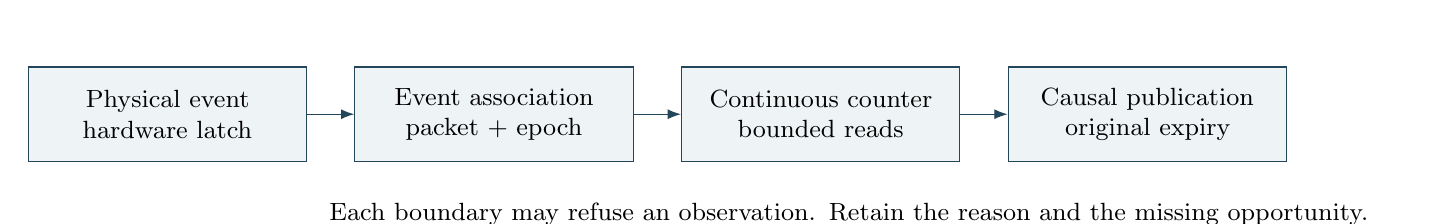
\begin{tikzpicture}[>=Latex,font=\small,node distance=6mm,
box/.style={draw=ink,fill=pale,align=center,text width=33mm,minimum height=12mm}]
\node[box](capture){Physical event\\hardware latch};
\node[box,right=of capture](identity){Event association\\packet + epoch};
\node[box,right=of identity](domain){Continuous counter\\bounded reads};
\node[box,right=of domain](map){Causal publication\\original expiry};
\draw[->,ink](capture)--(identity);
\draw[->,ink](identity)--(domain);
\draw[->,ink](domain)--(map);
\node[below=4mm of identity,anchor=north west,xshift=-29mm,align=center,text width=145mm]
{Each boundary may refuse an observation. Retain the reason and the missing opportunity.};
\end{tikzpicture}
\end{center}
\vspace{-6pt}
{\footnotesize Copyright \copyright\ 2026 Jonathan Yantis. Original paper, LaTeX and figure:
\href{https://creativecommons.org/licenses/by/4.0/}{CC BY 4.0}. Illustrative pseudocode: MIT. Referenced code retains its own license.
Author-review candidate; not submitted, peer reviewed or approved for library inclusion.}
\newpage

\section{Prior art and the current Zephyr boundary}
\subsection{Established techniques, different endpoints}
FTSP combined low-level timestamps, skew estimation and multihop distribution \cite{ftsp}. CheepSync brought low-level timestamps and compensation to BLE advertisers \cite{cheep}. BlueSync studied beacon-based synchronization and efficient tick adjustment \cite{blue}. Nordic's 2016 implementation used timers and programmable peripheral interconnect (PPI) to synchronize proprietary radio beacons alongside BLE \cite{nordic}. These works precede any claim based simply on a captured radio event, regression or a broadcast software clock.

Related systems also constrain the energy and operating-system claims. Virtual High-resolution Time combined fast active and slow sleeping clocks \cite{vht}. MicroSync combined hybrid timers and BLE communication scheduling; its high-accuracy configuration reports 272 ns mean absolute error and 319.2 ns standard deviation at 252.1 $\mu$W \cite{micro}. FLOPSYNC-3 introduced an RTOS virtual-clock interface and addressed the control consequences of applying correction at driver level \cite{flop}. These results have distinct references and statistics and are not ranked against PToB's PPS-map RMS.

\begin{center}\small
\begin{tabular}{L{.27\linewidth}L{.32\linewidth}L{.32\linewidth}}\toprule
Comparator & Established mechanism or endpoint & Remaining question for this study\\\midrule
Nordic timer demo \cite{nordic} & PPI, hardware timers, proprietary beacons & Correct association inside the Zephyr BLE controller lifecycle\\
Maiwald et al.\ \cite{maiwald} & Periodic-advertising multicast; reported maximum reaction difference 11 $\mu$s & Capture-domain and publication behavior, rather than application reaction alone\\
Zhou et al.\ \cite{zhou} & MPSL proprietary beacons; RSSI, traffic, cadence and connection-interval sweeps & Causal faults, false rejection and service coverage under matched workloads\\
Linux timestamping \cite{stamp} & Delayed TX timestamp joined to original packet identity & Small, bounded implementation on a constrained RTOS\\
Linux sequence counters \cite{seq} & Consistent reads; explicit warning about preempted writers & Reader refusal cost and interrupt-context constraints\\\bottomrule
\end{tabular}
\end{center}
\vspace{-4pt}
The 2026 Zhou preprint adapts Nordic's demo and measures physical GPIO differences under BLE traffic \cite{zhou}. Its timing beacons use proprietary radio mode, whereas this case study observes supported BLE periodic PDUs. A new workload sweep or a smaller selected average would therefore be insufficient differentiation. The proposed evaluation isolates event association, lifecycle and publication ordering. The Maiwald comparison above uses the author institution's abstract; its full experimental method was not available in this review.

\subsection{Build on the upstream mechanisms}
Zephyr merged shared precision-time arithmetic, clock operations, a PI controller and a PTP adapter on 28 September 2026 \cite{precision,stage2}. Its experimental subsystem leaves protocol policy and source handling to consumers. The broader architecture RFC already discusses counters, timestamp services and timescales \cite{architecture}. The PTP/gPTP roadmap is developing these boundaries incrementally \cite{roadmap}.

At this review date, draft PR~121471 provides scheduled output and PPS lifecycle work \cite{pps}. The roadmap's October input-capture discussion identifies IRQ ownership, bounded callbacks and low-rate polling as concrete requirements \cite{roadmap}. The documented periodic-advertising receive-info structure does not expose a physical hardware timestamp \cite{recv}; this observation concerns that interface, not every vendor controller API. Nordic's connected-time sample already exchanges anchor timestamps and event counters \cite{conn}. PToB's useful opportunity is to supply a supported BLE capture case, failure fixtures and measured costs to this existing work.

\newpage
\section{Associate the latch before interpreting the time}
\subsection{One counter, managed ownership}
The examined adapter requests the high-frequency clock through Zephyr's clock manager and uses a 32-bit TIMER3 at 16 MHz \cite{implementation}. The tick is 62.5 ns. PPS, radio ADDRESS and optional USB start-of-frame (SOF) capture into separate channels of that counter. A shared origin avoids a software bridge between those latches, but each peripheral still has its own endpoint delay and semantics.

Resource checks matter as much as the timer frequency. The adapter excludes the pinned controller's timer/PPI resources and leaves GPIOTE interrupt ownership with Zephyr. It does not commandeer the controller's RADIO or CLOCK tasks. A different SoC or controller configuration needs a new resource and interrupt audit; naming another spare timer is not sufficient.

\subsection{An event record is an association, not just a scalar}
The radio path retains the capture epoch, raw latch, controller owner, event counter, RF channel, direction and complete supported advertising bytes. Arm and completion hooks connect the latched event to the selected controller operation. Completion verifies the expected ADDRESS condition, completion status, receive CRC where applicable and accepted PDU shape before queue publication. The selected path is BLE 1M and rejects unsupported or ambiguous packet forms \cite{implementation}.

\begin{lstlisting}[caption={Illustrative contract; not a replacement driver.}]
arm(owner, pdu, event, channel, capture_epoch)
  require(supported_path && no_conflicting_capture)
  enable_owned_hardware_route()

complete(owner, done, crc)
  require(owner_matches_current_armed_operation)
  raw = read_latched_ADDRESS()
  disable_owned_route()
  require(done && ADDRESS_seen && receive_crc_ok_if_needed)
  require(supported_complete_PDU && queue_has_space)
  publish_copy(raw, epoch, owner, event, channel, direction, PDU)
\end{lstlisting}
An owner pointer is not a durable generation identifier: an allocator can reuse its address. Event counters wrap, and a controller can restart a train. Retain the counter epoch and the higher-level source/boot/path context; serialize closure and flush so old queued records cannot be admitted to a new lifecycle. If a future generic API uses an explicit generation token, document exactly which transition changes it.

\subsection{Close the operation before reusing its resources}
The capture queue has 16 entries. Queue overflow loses an observation; it does not authorize overwriting a timestamp and pretending the next packet supplied it. Disable refuses to report a clean close while a selected event remains armed. Stop/restart must resolve actual ownership and queued history before a new owner is admitted.

Raw ADDRESS is the present endpoint convention. TX and RX detector equivalence remains uncalibrated. Subtracting a PHY prefix can produce a register START coordinate, but does not measure an electrical launch or remove receiver delay. Keep raw capture, any normalization and calibration profile separate. A CRC establishes decoded packet integrity; it does not establish timestamp accuracy.

For delayed correction schemes, carry the original event identity through to the correction. Processing a later correction can update a map, but cannot refresh the original source permission simply by arriving later. A model's fit-reference instant, availability/activation instant and the physical event being evaluated are distinct. Past-event scoring must use a model available at that event, or explicitly report that causal reconstruction is unavailable \cite{archive,own}.

\newpage
\section{Extend the fine counter without inventing continuity}
\subsection{Separate counter extension from event reconstruction}
Let $r_i$ be a current 32-bit latch and $C_i$ its extended value. With validated continuity,
\[
 d_i=(r_i-r_{i-1})\bmod 2^{32},\qquad C_i=C_{i-1}+d_i .
\]
At 16 MHz the full wrap period is 268.435456 s. Unsigned subtraction alone cannot distinguish a short interval from that interval plus whole wraps. The serialized owner therefore requires timely extension, checks coarse monotonic progress and refuses excessive gaps, ambiguous deltas or integer overflow \cite{implementation}. Its one-second continuity policy is much shorter than the hardware wrap.

For an older captured event $r_e$, reconstruct against a validated \emph{current} latch $r_n$:
\[
 a=(r_n-r_e)\bmod 2^{32},\qquad C_e=C_n-a .
\]
The examined GM reader requires a matching epoch, a current base no more than 16,000,000 ticks behind the latch, and event age no greater than 4,000,000 ticks (250 ms). Check subtraction and extended range before conversion. Event age must be measured against current time, independently of the age of the last extension publication. An old base can otherwise make an already old queued event appear young.

\subsection{Bound the reader; keep one extension owner}
On a 32-bit MCU a 64-bit counter publication can tear. The GM reader obtains a sequence-validated group of 32-bit atomic fields: extended low/high words, raw base, epoch and continuity guard. It makes at most two attempts, then returns unavailable. It never becomes another wrap-extension owner.

Linux documents the familiar failure of an unbounded sequence-counter reader that interrupts its writer and spins waiting for that writer \cite{seq}. Bounded attempts adapt that established consistency pattern to a deadline-sensitive reader; they are not a new synchronization primitive. They bound this retry loop, not the whole call graph or memory-access latency. Writer serialization, memory ordering, compiler output and interrupt context still require platform-specific review.

The independent RTC1 observation is a negative continuity lease. It can reject an HF base whose extender has stalled; it does not supply fractional phase or replace a missing fine event. Its modular check relies on the accompanying extension/watchdog assumptions. A stopped or invalidated epoch remains closed even if an old publication arrives late. A new epoch requires an explicit lifecycle start.

\subsection{Bracket cross-domain reads and state their aperture}
Where kernel monotonic time and the HF domain must be related, the implementation brackets the HF read with kernel reads under a bounded IRQ critical section. Kernel reads are quantized: if $q_K$ bounds their downward quantization, the HF sample's kernel coordinate is enclosed by $[K_L,K_H+q_K)$ under the stated ordering assumptions. The bridge rejects a reported width above its 100 $\mu$s policy ceiling and restores the prior IRQ key on every path.

That ceiling is a refusal rule, not a measured normal duration or an RF error bound. The permission converter additionally shortens remaining lifetimes using a 200 ppm rate assumption and a 32 $\mu$s quantization margin; its header identifies the rate assumption as unverified. This bridge is not a calibrated phase map. Measure achieved aperture and interrupt blocking under workload. Its serialization assumptions exclude competing zero-latency access to the latch.

A disciplined map may be written $T=aC+b$, with an identified source and counter epoch. Nanosecond arithmetic improves its representation; it does not reduce the 62.5 ns capture grid or prove a physical uncertainty bound. Unknown reference, path or detector terms must remain unknown even when regression residuals are small.

\newpage
\section{A freshness race caused by publication ordering}
\subsection{New input can look like future input}
Freshness checks normally reject a sample timestamp $t_s$ when the processing time $t_q<t_s$. That is correct if both belong to one domain and $t_q$ was obtained after observing the sample. A stale loop timestamp violates that ordering assumption.

Consider the following synthetic schedule, in microseconds:
\begin{center}
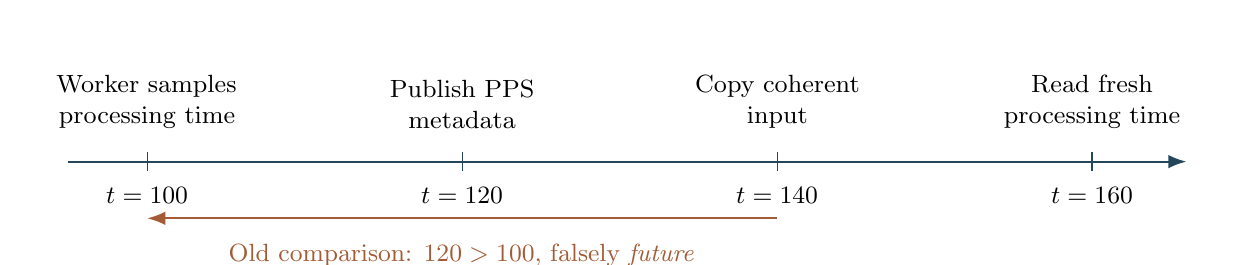
\begin{tikzpicture}[>=Latex,font=\small,x=1cm,y=1cm]
\draw[->,ink,thick](0,0)--(14.2,0);
\foreach \x/\t/\lab in {1/100/{Worker samples\\processing time},5/120/{Publish PPS\\metadata},9/140/{Copy coherent\\input},13/160/{Read fresh\\processing time}}{
 \draw[ink](\x,-.12)--(\x,.12);
 \node[above=3mm,align=center,text width=28mm]at(\x,0){\lab};
 \node[below=2mm]at(\x,0){$t=\t$};
}
\draw[->,accent,thick](9,-.72)--(1,-.72);
\node[below=2mm,text=accent]at(5,-.72){Old comparison: $120>100$, falsely \emph{future}};
\end{tikzpicture}
\end{center}
The metadata is coherent and the PPS is current, yet evaluation against $100$ rejects it. Repeating that pattern can reset source qualification or withdraw service. Reducing timer quantization or loosening a PLL gain cannot repair the ordering error. Increasing the permitted sample lifetime would hide it while weakening genuine expiry checks.

\subsection{Copy input, refresh the evaluation clock, preserve expiry}
The examined service copies source metadata and its physical map coherently. While holding that source lock, it obtains a fresh validated bridge and returns that same bridge to subsequent decisions \cite{implementation}. This orders the copied sample before the evaluation time while preventing concurrent publication from changing the copied state.

\begin{lstlisting}[caption={Fresh evaluation time does not grant a fresh source lifetime.}]
lock(source_owner)
  snapshot = copy_coherent_metadata_and_source_map()
  now = read_validated_kernel_HF_bridge()
unlock(source_owner)
require(now.valid && snapshot.counter_epoch == now.epoch)

require(snapshot.sample_time <= now.in_sample_domain)
require(now.in_sample_domain < snapshot.original_expiry)
return evaluate(snapshot, now)   // retain source and capture generations
\end{lstlisting}
The real production routine also evaluates the physical source at a later same-epoch capture and retains the distinction between its sample instant and the earlier bridge. The pseudocode states the ordering invariant, not exact executable instructions. Authentication, stop/fatal state and source generation remain separate gates. The original PPS/GNSS timestamps and their expiry horizons are not renewed by copying them.

\subsection{A regression with a narrow, useful claim}
The existing \src{gm7_source_order_test.c} constructs PPS and RMC publication between an earlier bridge and the coherent copy. Its 11 current cases include genuine future PPS, exact freshness expiry, invalid capture domain, epoch replacement, stopped/fatal source and unavailable UTC association. The runner can also accept an explicitly selected historical source fixture and demonstrate the old ordering failure \cite{implementation}.

This is a controlled production-body counterexample with fake kernel/capture boundaries. It identifies a possible software failure chain; it does not establish the physical cause of a historical field withdrawal. This draft does not report a fresh run of that native regression. The archive replay in Section~6 is a different check.

The broader rule is to acquire coherent state before the time used to judge it, then revalidate the applicable lifecycle and expiry. Apply it to watchdog snapshots, USB source maps and status publications as well as GNSS. Keep system scheduling on its monotonic clock; a synchronized or civil-time adjustment should not silently change timeout semantics.

\newpage
\section{Evidence, measurement and an adoptable artifact}
\subsection{Historical precision with its denominator intact}
The selected 12 October 2026 archive evaluates a causal software map at local physical PPS after two BLE links. Its 436 reference-valid usable observations have signed mean $-18.417431\ns$, bias-inclusive RMS $62.503871\ns$, absolute P99 $160.25\ns$ and maximum $191\ns$ \cite{archive}. The observation span is 601.5761865 s. The conservative nominal count is:
\[
602=\underbrace{436}_{\text{usable, reference valid}}+
\underbrace{65}_{\text{invalid reference}}+
\underbrace{3}_{\text{expired map, reference valid}}+
\underbrace{98}_{\text{unobserved}} .
\]
All 501 available-map causal observations, including invalid references, have RMS 3.929464 ms. That separate population preserves excursions; it is not a valid-reference accuracy estimate. Usable observed coverage is 72.425\% of nominal opportunities. Missing witnesses are unknown service intervals, not proof of an outage.

The historical calibration was a fixed empirical $+10{,}543\ns$ per received link. Its training inputs are absent from the public archive, so that calibration cannot be independently regenerated there. The experiment neither measures an output pin nor establishes calibrated UTC accuracy, and it cannot qualify the current GM7 source. Preparation reran \src{python3 tools/verify_v14.py}: the public numerical populations and archive checks passed. No new RF acquisition or physical timing comparison accompanied this draft.

\subsection{A controlled comparison that can establish benefit}
Use matched devices, cadence and predeclared observation windows. Compare callback timestamps, ISR timer reads, hardware capture, and the complete guarded path. Keep deliberately broken lifecycle/order variants in controlled fixtures. Test physical configurations only with their separately established operating scope.

\begin{center}\small
\begin{tabular}{L{.24\linewidth}L{.35\linewidth}L{.32\linewidth}}\toprule
Question & Controlled intervention & Required observation\\\midrule
Capture benefit & Callback versus ISR versus hardware latch & Signed bias, RMS, P99/maximum and scoring coverage\\
Association integrity & Delay, cancellation, owner reuse, overflow & Wrong acceptance, correct refusal and retained gaps\\
Continuity & Missed extension, wrap, stop/restart, epoch change & Alias prevention, recovery and reader attempts\\
Freshness ordering & Publish between old \emph{now} and input copy & False future rejection and qualification resets\\
Operating cost & USB, display, logging and BLE control load & Aperture, IRQ blocking, queue occupancy and availability\\\bottomrule
\end{tabular}
\end{center}
\vspace{-4pt}
For every scheduled query, record the service verdict and witness eligibility separately. Report returned-valid availability, independently scoreable coverage and conditional error statistics. A conservative observed within-budget fraction is
\[
 \frac{\#\{\text{valid output, eligible witness, }|e|\le\epsilon\}}
      {\#\{\text{all scheduled opportunities}\}} .
\]
Unknown opportunities remain identified alongside that fraction; they are not proven failures or successes. Withholding every difficult sample cannot count as improved timing service. Measure energy only with an actual power instrument, and freeze calibration before held-out runs or devices.

\subsection{Practical conclusion and remaining work}
Package a small capture example, explicit clock/event/epoch contracts, controlled failure fixtures, source pins and complete denominators. Retain the pinned 4.1 baseline and evaluate a separately pinned current Zephyr revision before claiming an upstream deficiency. Attribute the existing Zephyr/ZMK backports; successful compilation or simulator checks add no physical qualification.

The present result is an inspectable engineering account, not a new synchronization primitive. Its useful next contribution is to demonstrate how much correct event association, continuity checks and publication ordering improve the accuracy--availability--cost tradeoff. That evidence could inform Zephyr's ongoing event-capture work and give application engineers a reproducible route from a hardware latch to usable time.

\newpage
\begingroup
\fontsize{9}{10.6}\selectfont
\setlength{\parskip}{1pt}
\begin{thebibliography}{99}
\setlength{\itemsep}{3pt}
\bibitem{implementation} J. Yantis, \emph{PToB T096 source and dependency lock}, repository revision \pin, 1 Nov. 2026. \href{https://github.com/yantisj2/PToB}{Repository}. Companion \src{edition.json} identifies the examined files; code licenses are preserved. This review does not assert that the local revision is a published release.
\bibitem{precision} Zephyr Project, \emph{Precision Timing}, experimental subsystem documentation. \href{https://docs.zephyrproject.org/latest/kernel/precision_timing.html}{Documentation}.
\bibitem{architecture} Zephyr Project, \emph{RFC: Proposal for a Precision Clock Subsystem Architecture}, issue 76335, opened 2024. \href{https://github.com/zephyrproject-rtos/zephyr/issues/76335}{Architecture RFC}.
\bibitem{stage2} Zephyr Project, \emph{Reusable precision timing infrastructure for PTP and gPTP}, PR 115363, merged 28 Sept. 2026. \href{https://github.com/zephyrproject-rtos/zephyr/pull/115363}{Merged implementation}.
\bibitem{roadmap} Zephyr Project, \emph{RFC: Roadmap for PTP/gPTP}, issue 107837, 2026; including the 23 Oct. input-capture use case. \href{https://github.com/zephyrproject-rtos/zephyr/issues/107837}{Roadmap and discussion}.
\bibitem{pps} Zephyr Project, \emph{Scheduled output and PPS service}, draft PR 121471, 2026. \href{https://github.com/zephyrproject-rtos/zephyr/pull/121471}{Proposed implementation}.
\bibitem{ftsp} M. Maroti, B. Kusy, G. Simon and A. Ledeczi, \emph{The Flooding Time Synchronization Protocol}, SenSys, pp. 39--49, 2004. \href{https://doi.org/10.1145/1031495.1031501}{doi:10.1145/1031495.1031501}.
\bibitem{cheep} S. Sridhar, P. Misra, G. S. Gill and J. Warrior, \emph{CheepSync: A Time Synchronization Service for Resource Constrained Bluetooth Low Energy Advertisers}, 2015; revised 2016. \href{https://arxiv.org/abs/1501.06479}{arXiv:1501.06479}.
\bibitem{blue} F. Asgarian and K. Najafi, \emph{BlueSync: Time Synchronization in Bluetooth Low Energy With Energy-Efficient Calculations}, IEEE Internet of Things Journal, 9(11), pp. 8633--8645, 2022; online 2021. \href{https://doi.org/10.1109/JIOT.2021.3116921}{doi:10.1109/JIOT.2021.3116921}. Publisher abstract reviewed.
\bibitem{nordic} Nordic Semiconductor (Audun), \emph{Wireless timer synchronization among nRF5 devices}, 12 July 2016. \href{https://devzone.nordicsemi.com/guides/short-range-guides/b/bluetooth-low-energy/posts/wireless-timer-synchronization-among-nrf5-devices}{Vendor article};
\href{https://github.com/nordic-auko/nRF5-ble-timesync-demo}{implementation and NCS sample}.
\bibitem{micro} R. Ohara et al., \emph{MicroSync: Sub-Micro Second Accuracy Wireless Time Synchronization Service}, IEEE Access, 12, pp. 124478--124494, 2024. \href{https://doi.org/10.1109/ACCESS.2024.3446668}{doi:10.1109/ACCESS.2024.3446668};
\href{https://da.lib.kobe-u.ac.jp/da/kernel/0100491658/0100491658.pdf}{version of record}.
\bibitem{zhou} Z. Zhou et al., \emph{Multiprotocol Wireless Timer Synchronization for IoT Systems}, author preprint, 8 Apr. 2026. \href{https://arxiv.org/abs/2604.07199}{arXiv:2604.07199}.
\bibitem{vht} T. Schmid, P. Dutta and M. B. Srivastava, \emph{High-Resolution, Low-Power Time Synchronization: an Oxymoron No More}, IPSN, 2010. \href{https://people.eecs.berkeley.edu/~prabal/pubs/papers/schmid10vht.pdf}{Author-hosted paper}.
\bibitem{flop} A. Sorrentino, F. Terraneo and A. Leva, \emph{Efficient Abstraction of Clock Synchronization at the Operating System Level}, NG-RES, pp. 4:1--4:11, 2023. \href{https://doi.org/10.4230/OASIcs.NG-RES.2023.4}{doi:10.4230/OASIcs.NG-RES.2023.4}.
\bibitem{seq} Linux Kernel, \emph{Sequence counters and sequential locks}. \href{https://cdn.kernel.org/doc/html/latest/locking/seqlock.html}{Kernel documentation}.
\bibitem{stamp} Linux Kernel, \emph{Timestamping}, including delayed TX timestamp/packet association. \href{https://cdn.kernel.org/doc/html/latest/networking/timestamping.html}{Kernel documentation}.
\bibitem{recv} Zephyr Project, \emph{bt\_le\_per\_adv\_sync\_recv\_info}, API documentation identified as 4.5.0-rc3. \href{https://docs.zephyrproject.org/latest/doxygen/html/structbt__le__per__adv__sync__recv__info.html}{Receive-report fields}.
\bibitem{maiwald} T. Maiwald et al., \emph{Timing Deviations in Wireless Networks using Bluetooth Periodic Advertising}, I2MTC, pp. 1--6, 2022. \href{https://doi.org/10.1109/I2MTC48687.2022.9806632}{doi:10.1109/I2MTC48687.2022.9806632};
\href{https://cris.fau.de/publications/269905857/}{author institution abstract reviewed}.
\bibitem{archive} J. Yantis, \emph{V14 successor research: 12 October 2026}, selected evidence, summary and verifier. \href{https://github.com/yantisj2/PToB/tree/main/evidence/v14/2026-10-12}{Evidence collection}; \src{tools/verify_v14.py}. Historical application 0.14.43; no current-firmware acceptance implied.
\bibitem{own} J. Yantis, \emph{PToB Viability: Rooted BLE Timing Meshes for Heterogeneous Edge Networks}, research draft, 30 Oct. 2026. \href{https://github.com/yantisj2/PToB/blob/main/papers/ptob-viability-preprint.pdf}{Manuscript}; see also the separate 12 Oct. boundary-clock study and 24 Oct. ESP32-S3 implementation guide in the repository paper catalogue.
\bibitem{conn} Nordic Semiconductor, \emph{Bluetooth: Connection time synchronization}, nRF Connect SDK documentation. \href{https://nrfconnectdocs.nordicsemi.com/ncs/latest/nrf/samples/bluetooth/conn_time_sync/README.html}{Connection-anchor sample}.
\end{thebibliography}
\smallskip
\noindent\textit{Review boundary.} Online sources were reviewed on 1 November 2026. Development documentation, issue bodies and PR status may change. This is a targeted primary-source review, not a proof of priority. The companion source ledger records access limitations. Codex assisted with research, drafting and artifact checks; Jonathan Yantis is the author responsible for review and any later publication.
\endgroup
\end{document}
